\documentclass[a4paper]{article}
\usepackage[francais]{babel}
\usepackage[T1]{fontenc}
\usepackage[applemac]{inputenc}
\usepackage{geometry}
\usepackage{graphicx}
\usepackage[colorlinks=true]{hyperref}
\hypersetup{urlcolor=blue,linkcolor=black,colorlinks=true} 
\usepackage{algorithm,algorithmic}
\usepackage{listings}
\usepackage{amssymb}
\usepackage{setspace}
\usepackage{listings}
\usepackage{lscape}
\usepackage{multimedia}
\usepackage[toc,page]{appendix} 
\usepackage[final]{pdfpages} 


\pagestyle{headings}
\thispagestyle{empty}
\geometry{a4paper,twoside,left=2.5cm,right=2.5cm,marginparwidth=1.2cm,marginparsep=3mm,top=2.5cm,bottom=2.5cm}
\begin{document}
\large
\setlength{\parskip}{10mm plus2mm minus2mm}
\setlength{\evensidemargin}{-2cm}
\setlength{\textwidth}{530pt}
\setlength{\parindent}{0cm}

21 janvier 2012 \hfill M1 Informatique


{\centering \Large \bfseries Analyse et conception d'algorithmes �conomes en �nergie dans les r�seaux de capteurs \par}

{�tudiants :
\begin{description}
\item Chlo� DESDOUITS \hfill chloe.desdouits@etud.univ-montp2.fr
\item Zahir KALI \hfill zahir.kali@etud.univ-montp2.fr
\item Rabah LAOUADI \hfill rabah.laouadi@etud.univ-montp2.fr
\item Samuel ROUQUIE \hfill samuel.rouquie@etud.univ-montp2.fr
\item
\end{description}

Encadrante : Anne-Elisabeth Baert
\par}

{{\bfseries Articles lus par le groupe entier}

\begin{itemize}
\item \emph{Dynamic Localized Broadcast Incremental Power Protocol and Lifetime in Wireless Ad Hoc and Sensor Networks} : Julien Champ, Anne-Elisabeth Baert and Vincent Boudet
\item \emph{Lifetime in Wireless Sensor Networks} : Julien Champ, Cl�ment Saad, Anne-Elisabeth Baert
\end{itemize}
}


{{\bfseries T�ches}

Chlo� :\\
Lecture de \emph{Energy conserving routing in wireless ad-hoc networks} : J.-H.Chang, L.Tassiulas. R�flexion et programmation.


Zahir :\\
Lecture de \emph{Wireless sensor networks: a survey} : I. F. Akyildiz, W. Su, Y. Sankarasubramaniam, and E. Cayirci. R�flexion et programmation.

Rabah :\\
Lecture de \emph{Maximizing system lifetime in wireless sensor networks} : Q.Dong. R�flexion et programmation.

Samuel :\\
\emph{Minimum energy mobile wireless networks} : V. Rodoplu and T.H. Meng. R�flexion.

\par}

\begin{landscape}

\begin{figure}
\centering
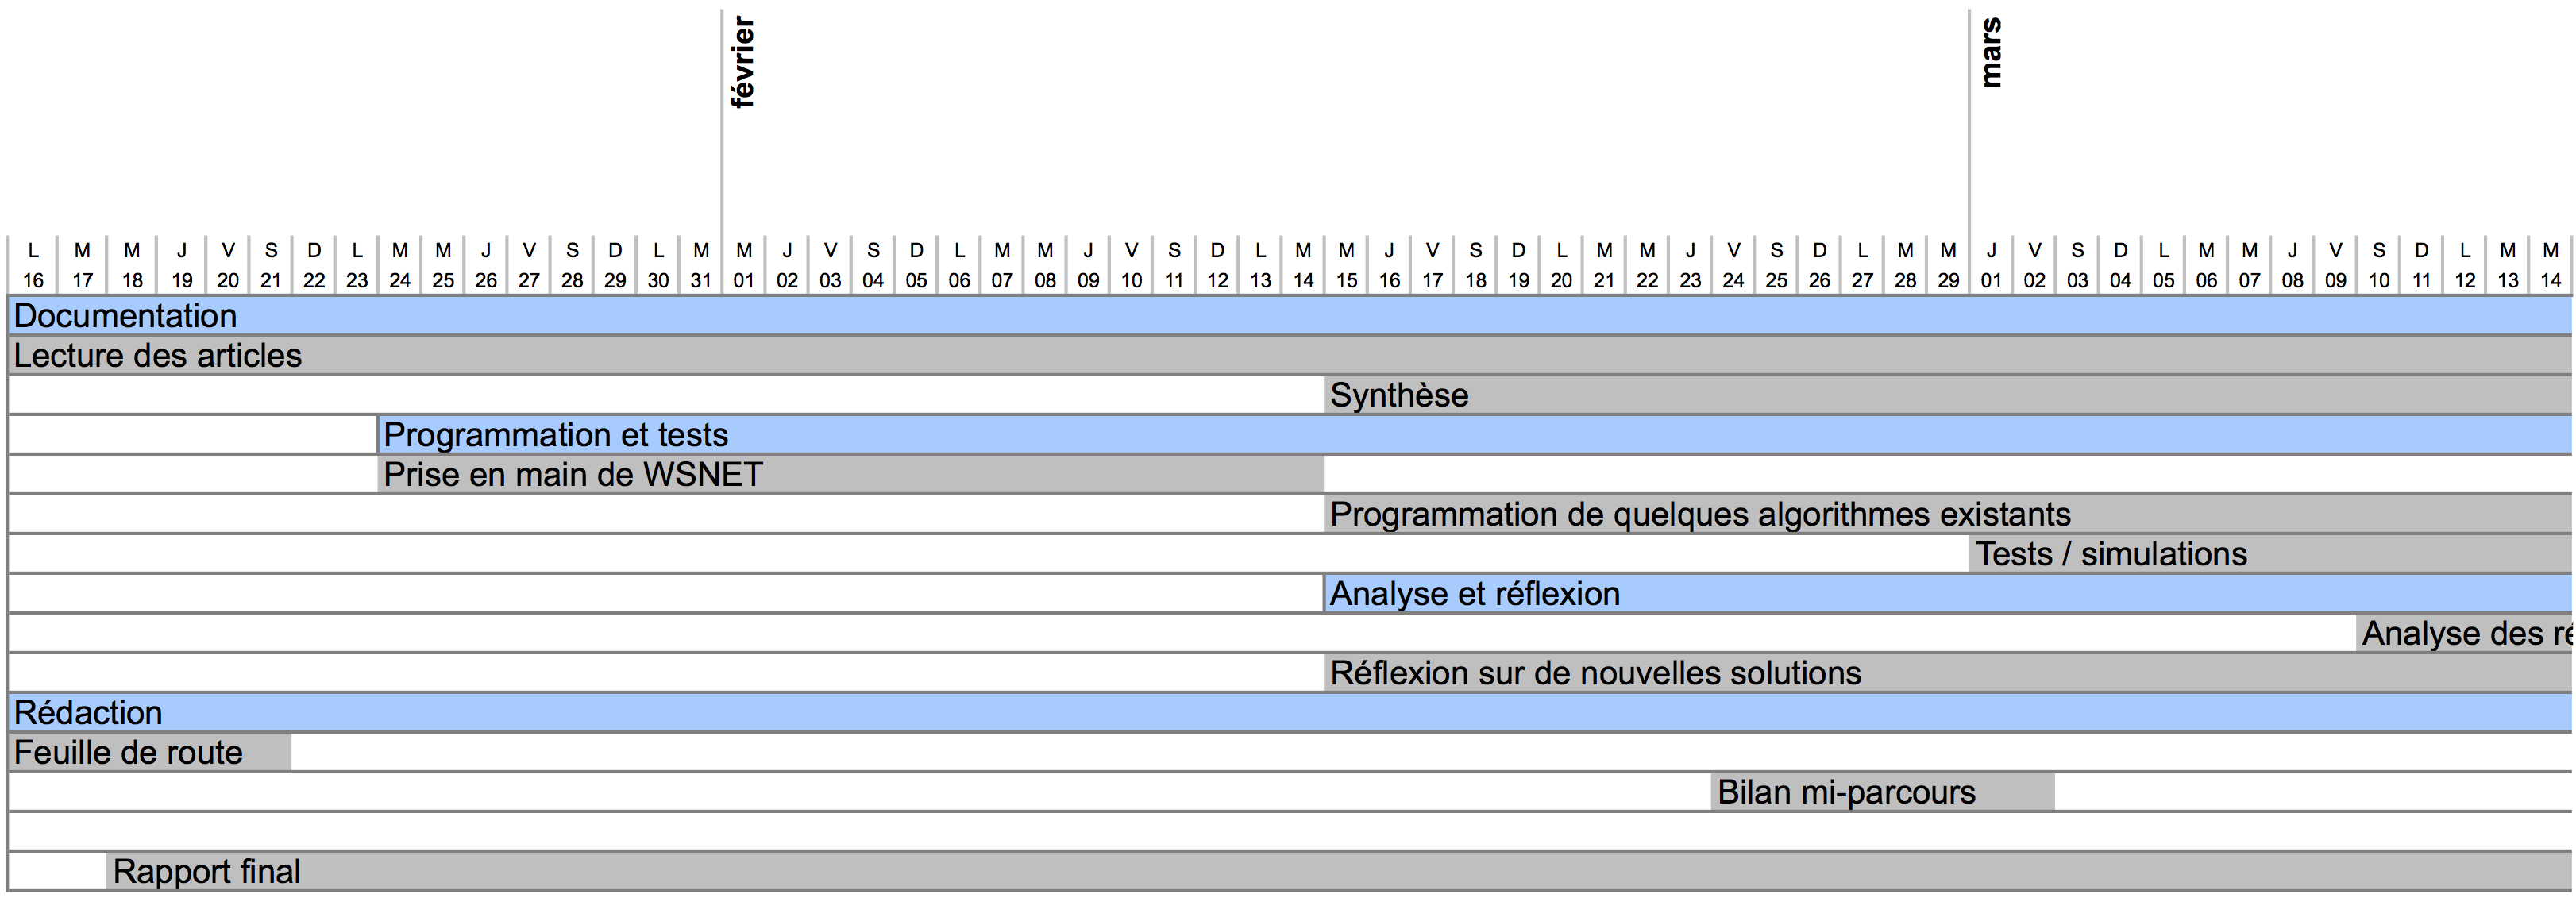
\includegraphics[scale=0.9]{diagramme}
\end{figure}

\begin{figure}
\centering
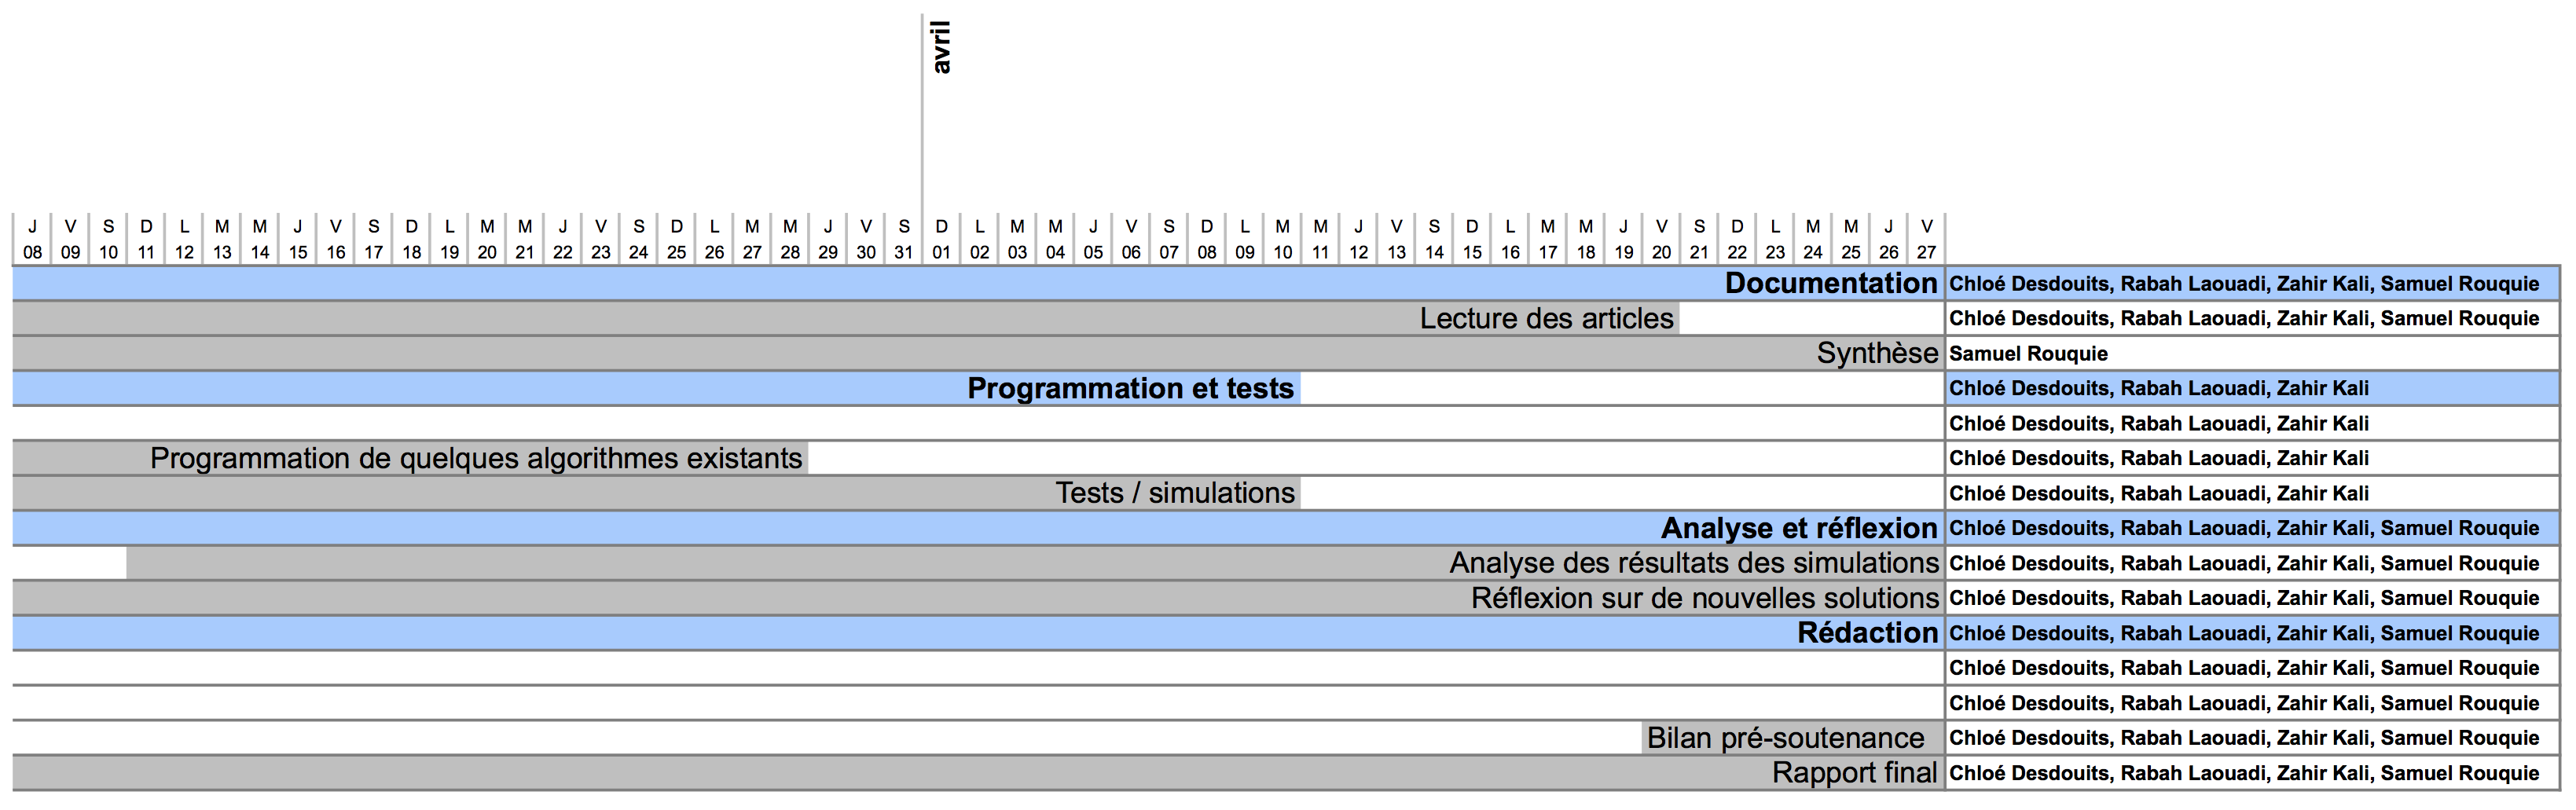
\includegraphics[scale=0.9]{diagramme2}
\end{figure}

\end{landscape}

\end{document}
